% Section content template for individual Educative lessons
% This file contains the actual content for a specific section
% Generated from Educative API section content

% Section: Sequence Diagram for the Meeting Scheduler
% Section ID: 4728022133637120
% Section Slug: sequence-diagram-for-the-meeting-scheduler
% Generated: 2025-12-12T13:06:38.704805

Sequence diagrams are a great way to understand the interactions between different entities and objects in the system. There can be multiple sequence diagrams for our meeting scheduler; here, we focus on the flow for scheduling a new meeting.
\\
In this lesson, we will create sequence diagrams for the following interactions:

\begin{itemize}
\item
\protect\phantomsection\label{yKxI54WXdqEVVEGwrxRhD}
\textbf{Schedule a meeting:}~The meeting organizer schedules a meeting time for some attendees.
\item
\protect\phantomsection\label{O1Moad9ZhBSh6UBaz0oDG}
\textbf{Sequence challenge:}~The meeting organizer cancels a scheduled meeting.
\end{itemize}

\subsection{Schedule a meeting}\label{RAjpkXXrc0ZzS0bqgtYrj}
\\
The sequence diagram to schedule a meeting should have the following actors and objects that will interact with each other:

\begin{itemize}
\item
\protect\phantomsection\label{N3XI3umAtJzz_PPxEicOv}
\textbf{Actor:} \texttt{Organizer}
\item
\protect\phantomsection\label{-dtDYbYO4tru1V1OMInsz}
\textbf{Objects:} \texttt{MeetingScheduler}, \texttt{MeetingRoom}, \texttt{Meeting}, and \texttt{Calendar}
\end{itemize}
\\
The steps in the schedule meeting interaction are listed below:

\begin{enumerate}
\item
\protect\phantomsection\label{3uAt2xUAStKUOXEfi7-5L}
The organizer requests that a meeting be scheduled, specifying the list of participants, the time interval, and the meeting subject.
\item
\protect\phantomsection\label{CfOmqpnlqpBfNkt8X2J-G}
The \texttt{MeetingScheduler} checks for the availability of a suitable \texttt{MeetingRoom} for the given interval and required capacity.
\item
\protect\phantomsection\label{QG7M3pJnqyxxCmTM1r2lF}
If a room is available:

\begin{enumerate}
\item
The \texttt{MeetingScheduler} books the room for the requested interval.
\item
The \texttt{MeetingScheduler} creates a new \texttt{Meeting} and assigns the organizer and all participants. By default, all participant statuses are set to ``PENDING.''
\item
The \texttt{MeetingScheduler} adds the new meeting to each participant's calendar (including the organizer).
\item
The \texttt{MeetingScheduler} sends an invitation notification to each participant.
\item
The \texttt{MeetingScheduler} informs the organizer that the meeting has been scheduled successfully.
\end{enumerate}
\item
\protect\phantomsection\label{n3sAPIembAXGEUR8YRdNx}
Else, if no room is available:

\begin{enumerate}
\item
The \texttt{MeetingScheduler} informs the organizer to select another meeting time or room.
\end{enumerate}
\end{enumerate}
\\
Based on the order above, the sequence diagram for scheduling a meeting in the meeting scheduler system is given below:

\begin{figure}[htbp]
 \centering
 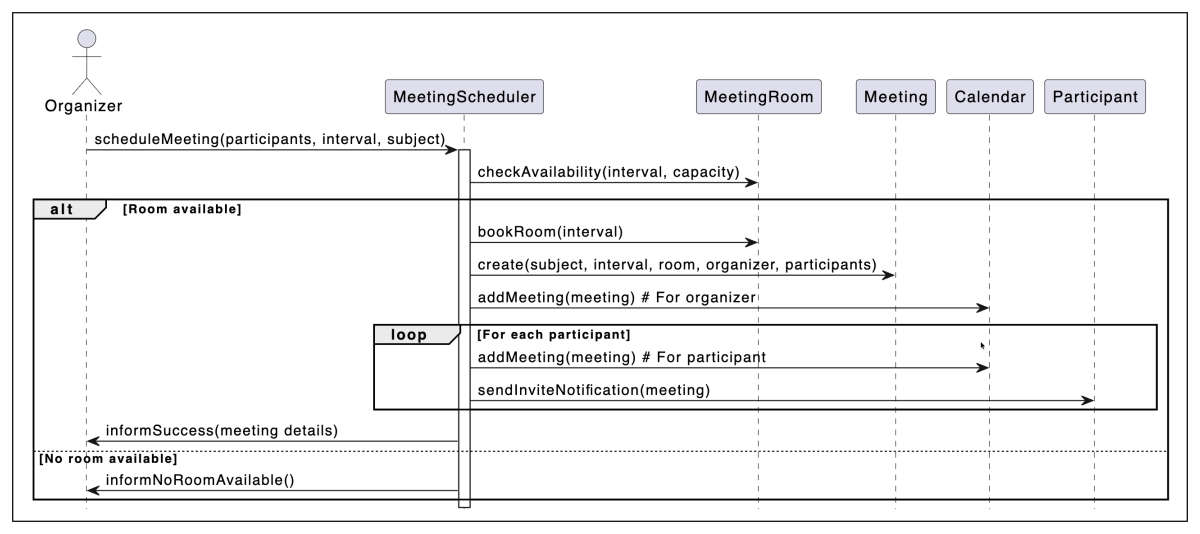
\includegraphics[width=0.5\textwidth]{Images/chapter_13/section_4728022133637120/4685128994258944.png}
 \caption{The sequence diagram for scheduling a meeting}
\end{figure}

\subsection{Sequence challenge: Cancel meeting}\label{bFv7qW5RSn6Zv6FSwydlR}
\\
You'll help us to complete a sequence diagram for the cancel meeting interaction. A skeleton of the cancel meeting sequence diagram is provided below:

\begin{figure}[htbp]
 \centering
 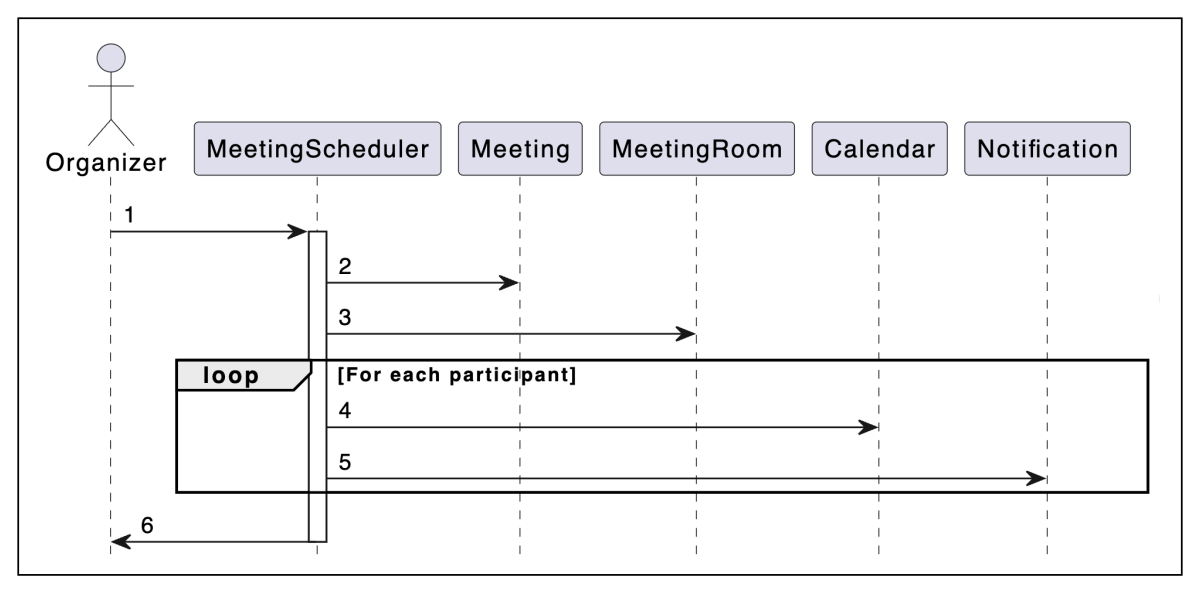
\includegraphics[width=0.5\textwidth]{Images/chapter_13/section_4728022133637120/5459046080315392.png}
 \caption{The sequence diagram for canceling a meeting}
\end{figure}

Notice that the arrows in the diagram above are numbered from 1 to 7. The message boxes shown below are the messages to be exchanged between the actor(s) and object(s). Can you rearrange the messages below in the correct sequence in order they should appear in the skeleton of the sequence diagram given above?
\begin{quote}
\textbf{Note:} If you're stuck, click the ``Show Solution'' button.
\end{quote}


Alternatively, you can click the ``Show complete diagram'' button below to see the complete sequence diagram for the cancel meeting interaction.

Next, let's look at the activity diagrams for the meeting scheduler to understand the control flow of the system.

% End of section content